\section{Инсталиране на продукта}

За инсталиране на продукта може да се клонира хранилището на проекта в GitHub.

Линк: https://github.com/Jobche/Jobche-BE

За да се клонира първо трябва да е инсталиран git клиента за терминал и да се изпълни командата:

``git clone https://github.com/Jobche/Jobche-BE''

Това ще клонира целия проект в текущата директория.

\section{Използване на продукта}

\subsection{Стартиране}
За стартиране на продукта има няколко варианта, но най-лесните са:
\begin{itemize}
    \item Ако имате инсталиран IntelliJ IDE просто отворете проекта в него и натиснете зелената стрелка горе-вдясно на прозореца. Това ще стартира проекта.
    \item През конзолата може да се стартира като се влезне в директорията на проекта и се напише ``./gradlew bootRun''. Това ще изпълни gradle Task, който стартира целия проект.
\end{itemize}

\subsection{Използване}
При стартиране на проекта на локална машина може да се достъпи на URL:localhost:8080. Това е основния линк, от който могат да се достъпят крайните точки (Примерно localhost:8080/users/create е линка за създаване на потребител). Но най лесният начин за използване ако желаете единствено да го пробвате е чрез \textbf{Swagger}.
На линк ``localhost:8080/swagger-ui.html'' може да се достъпи Swagger интерфейса на проекта.

\begin{figure}[h]
    \centering
    \makebox[\textwidth][c]{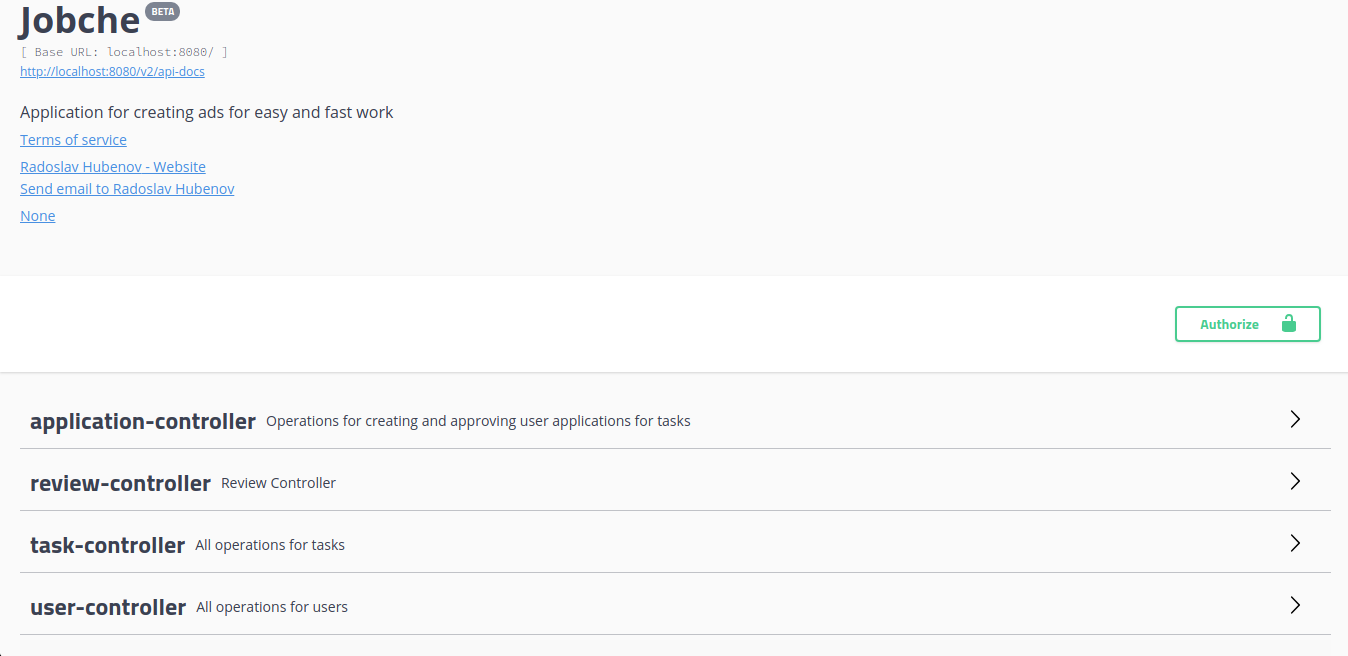
\includegraphics[width=1\textwidth]{images/swagger_ui.png}}%
    \caption{}
    \label{fig:swagger_ui}
\end{figure}

На фигура \ref{fig:swagger_ui} е показан част от интерфейса на Swagger. През него могат да се изпълняват заявки директно към продукта, но основната цел е за документиране на крайните точки.

Когато се натисне върху един от контролерите чекмеджето се отваря за да покаже всяка крайна точка, която този контролер съдържа. 

\begin{figure}[h]
    \centering
    \makebox[\textwidth][c]{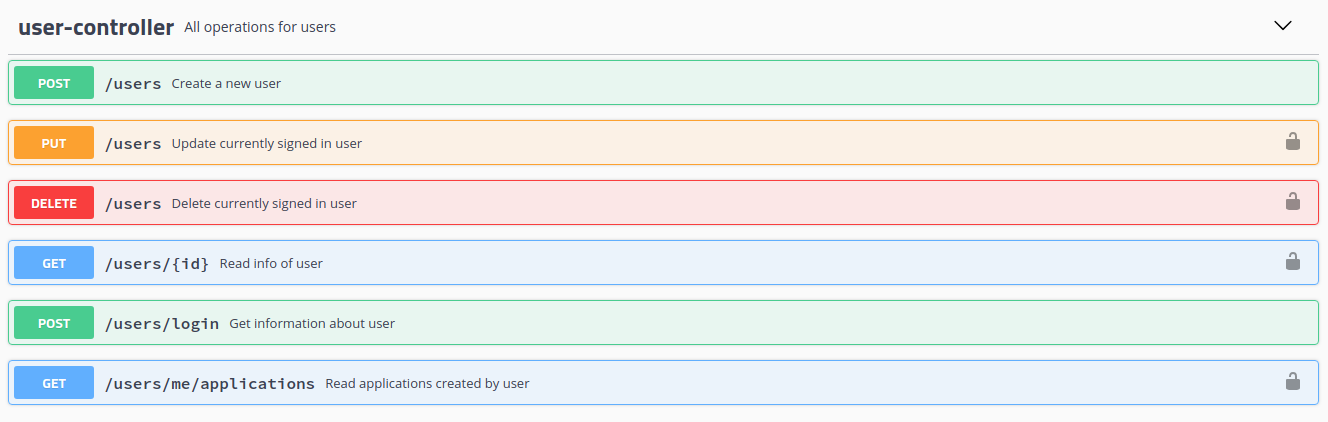
\includegraphics[width=1\textwidth]{images/swagger_users.png}}%
    \caption{}
    \label{fig:swagger_users}
\end{figure}

От тук клиент може да открие всичката му необходима информацип за достъпните крайни точки. Описана е функцията, която те извършват, както и JSON тялото, което очакват и което връщат.

Отваряйки крайна точка виждаме полетата, които се изискват, както и възможните отговори, които можем да получим. Позволение на това всеки, който желае да използва API-то за да изработи приложение спрямо него може лесно да разбере всичката нужна информация.

\begin{figure}[h]
    \centering
    \makebox[\textwidth][c]{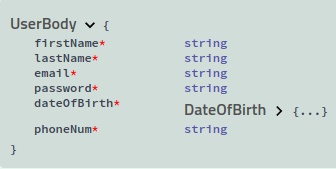
\includegraphics[width=0.5\textwidth]{images/swagger_user_model.png}}%
    \caption{}
    \label{fig:swagger_ui}
\end{figure}

Показан ни е обекта, който крайната точка очаква да получи както и кои от тях са задължителни. Всяко поле, което има звезда над името си е задължително.

Натискайки \textbf{Try it out} и след това \textbf{Execute} се изпълнява заявка с подаденото JSON тяло, на която заявка се връща и отговора от сървъра.